\chapter{ACTIVITY REPORT}
\section{Business Process in Company}
Business process that takes place in GSIT (Strategic Information Technology Group) in doing the process of production from start until it released are:
\begin{enumerate}
\item Requirement Assessment

Assessment of the need of latest technology required for BCA is typically done by Business Team or Fund Development Division  that doing the researches and compares the other bank technologies to emerge new business idea.

\item Sharing and Offering
The business idea then being discussed and proposed by GSIT in order to be applied in BCA. From that, the idea will be translated into other features or facilities in that application. Each feature is discussed in detailed until in its function and design.

\item IT Assessment

In this stage, GSIT will present its opinion about design that had been proposed and its technical implementation. Sometimes a very good design, not necessarily technically applicable. Depends on platform decision or operation system that will be used. Gathering requirements and making flow diagram from each feature also be done in this step.

\item Business Process

In making business process, GSIT is assisted by Business System Procedure (BSP) Division. GSIT and BSP will discuss together about each feature in detail, and repeating the gathering requirements process due to the possibility of increasing or more specific requirements is needed.

In this stage also, timeline or scheduling will be made together with Client and Application (CLA) Division to determined how long time to developing the application is needed. In making the schedule, usually deadline negotiation  is done in order to avoid over-time and also not too fast, so the product is really qualified and meet customer's desire.

\item Develop and Testing

The method that used in this developing stage is Scrum. Scrum is a framework for solving complex and adaptive problems, and at the same time, producing high value product with creativity and productivity. This technique makes the job become more organized and more detailed.\\

For instance, in an application to be built, there are 4 features in it. The team will work on one feature first, and then sent it to Client and Application Division for testing process. While the feature is being tested, GSIT worked on the second feature in order to do that feature testing immediately. And so on until all four feature had been completed. If in a feature there is a flaw or error during testing, it will be returned to GSIT for repairs.\\

After all features are done, it will be tested once more thoroughly (whole features testing) to check the perfection of built application. Then will be made certification and complementary documents before the application is released.

\item Publish

In publish stage, application that has been made is ready to be use. The application will be reviewed again about its function and the purpose of the application is built. If its an internal application, it will be given or distributed to internal company. But if its public or mass application, it will be published on Google Play Store and App Store.

\end{enumerate}
\section{Activities Performed According Learning Plan}
According to learning plan, the main jobs of the author is doing the migration of ETL jobs. The author's main tools to develop these projects is Informatica. Informatica consists of 4 software, Informatica Designer (Is used to develop the mapping), Informatica Workflow (Is used to develop the workflow), Informatica Monitor (To monitor every workflow that had/is running), and Informatica Repository (Manage the repository and data inside Informatica) On doing this, there are view process needs to be done step by step.

\subsection{Develop Mapping}
\begin{figure}[H]
\centering
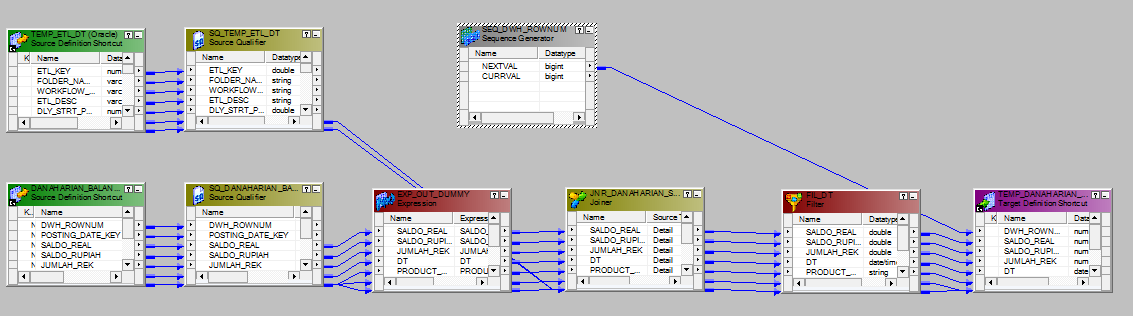
\includegraphics[width=\linewidth]{mapping-for-report.png}
\caption{Mapping in Informatica}
\label{fig:mapinfa}
\end{figure}

Figure~\ref{fig:mapinfa} shows the example of mapping in Informatica tools (ETL software). The mapping was the result of converted query of ETL jobs in old ETL software, Sagent tools (Figure~\ref{fig:saginfa}). To be able to develop mapping in Informatica, the author needs to understand the query and be able to read the ETL jobs in Sagent tools. Mapping is used to simplify executing the query.\\

In Informatica tools, transformation tools is used as a replacement of query. Each function on query has it's own transformation. For instance, sort, join, or rank function are different and has their own transformation.

\begin{figure}[H]
\centering
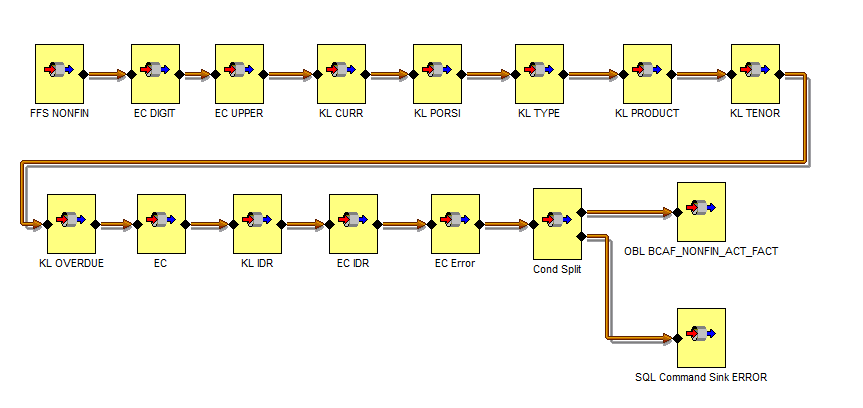
\includegraphics[width=\linewidth]{sagent-for-report.png}
\caption{Mapping in Sagent}
\label{fig:saginfa}
\end{figure}

\subsection{Mapping review}
After mapping was developed, a review is needed before go to the next step. The review process is done not only one times. The mapping will always be reviewed until it completely meets the requirement to go to the next step. Mapping that has been made will be reviewed in 2 steps.

\paragraph{Review by PIC}
Each mapping on the project will be reviewed by each PIC that has been assigned on that project. The PIC usually only briefly check the logic of mapping. Later will be checked by script more detail.

\paragraph{Review by script}
After being reviewed by PIC, mapping needs to be checked with script. The script is already been made and reusable (which means can be used for every mapping). The script usually tend to check settings and naming on mapping.

\subsection{Develop Workflow}

\begin{figure}[H]
\centering
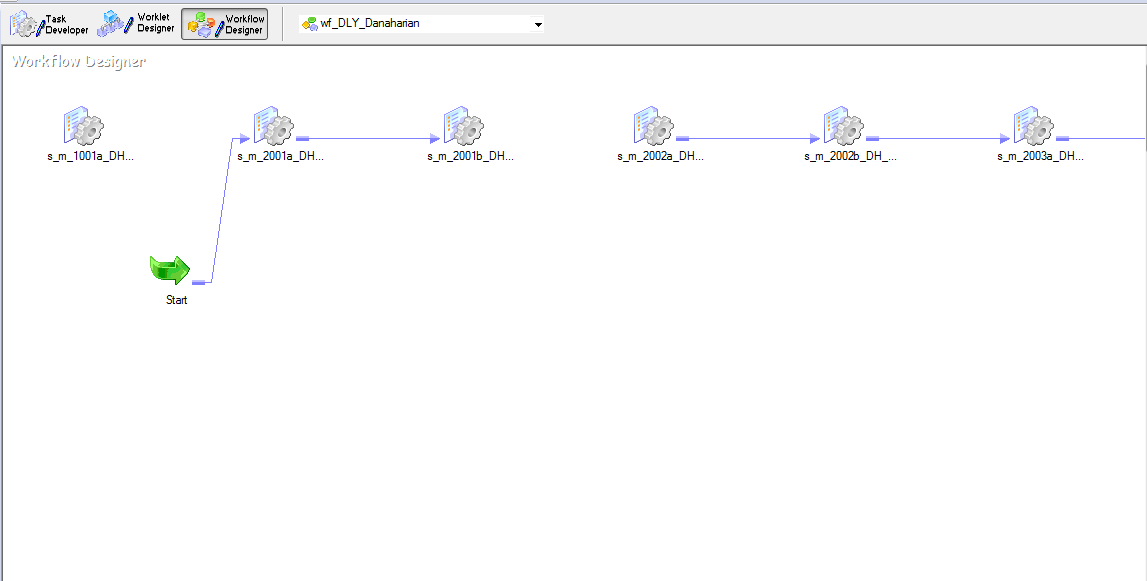
\includegraphics[width=\linewidth]{wf-for-report.png}
\caption{Workflow in Informatica}
\label{fig:wfinfa}
\end{figure}

The next step after finished develop the mapping of ETL is to create the workflow. A workflow usually consists of sessions and other task, but most of all is sessions. The session is made based on the mapping that has been made. One session is only made for one mapping.\\

From Figure~\ref{fig:wfinfa}, can be seen the green arrow is the start of the flow. Each session is linked by a connector. After the flow has been made, the configuration need to be set. Usually, the configuration that needs to be set is the workflow configuration and configuration of each session.

\begin{figure}[H]
\centering
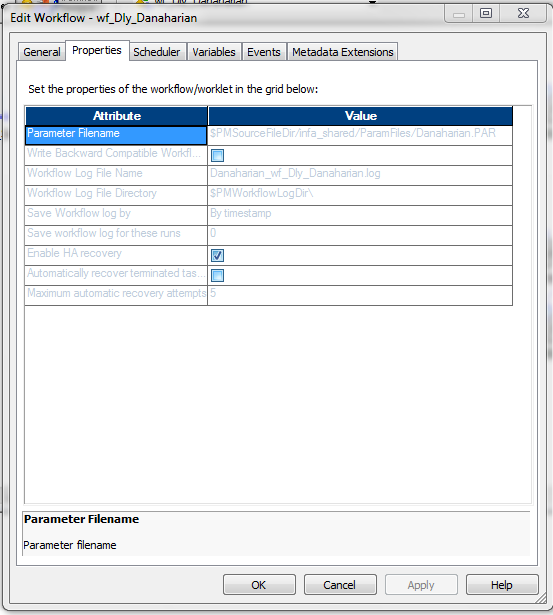
\includegraphics[width=\linewidth]{setting-in-wf.png}
\caption{Workflow setting in Informatica Workflow}
\label{fig:setwf}
\end{figure}

Figure~\ref{fig:setwf} is a glimpse of settings that needs to be configured in workflow settings. There are 6 tabs in there, but usually only 4 tabs that will be configured. Each needs to be set correctly before go to the next step.

\begin{figure}[H]
\centering
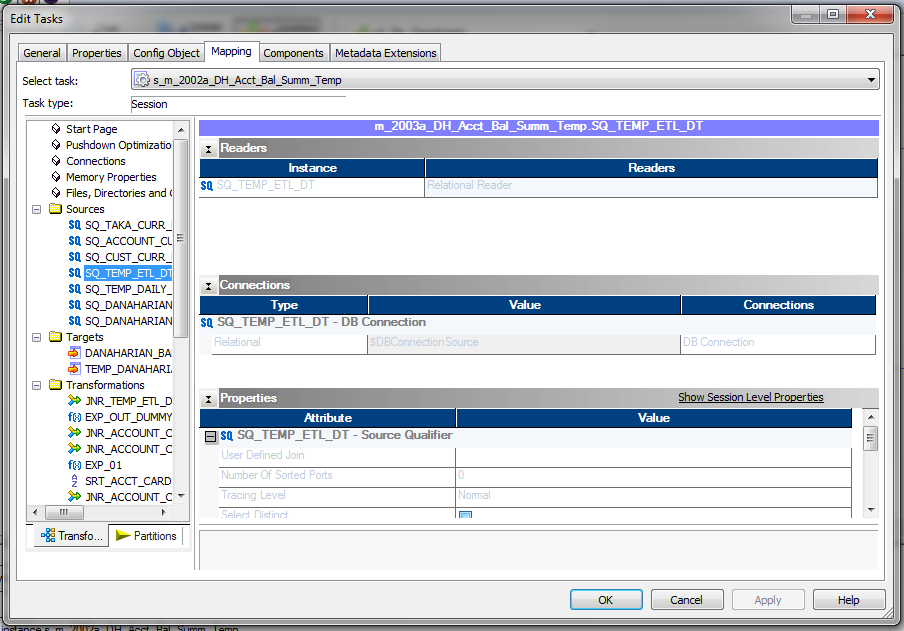
\includegraphics[width=\linewidth]{setting-in-ses.png}
\caption{Session setting in Informatica Workflow}
\label{fig:setses}
\end{figure}

After configuring workflow, each session has its own configuration. Figure~\ref{fig:setses} is a glimpse of settings that needs to be configure on each session before execute the workflow. Each needs to be set correctly, or else it will throw an error/errors.

\subsection{SIT}
SIT or System Integration Test is a process where we test the workflow by running the job that has made and make sure it has no flaws and the jobs executed completely. Job in here means the ETL job that has been converted from query or old ETL mapping. The session that has been made and setup consist of these ETL jobs.

\begin{figure}[H]
\centering
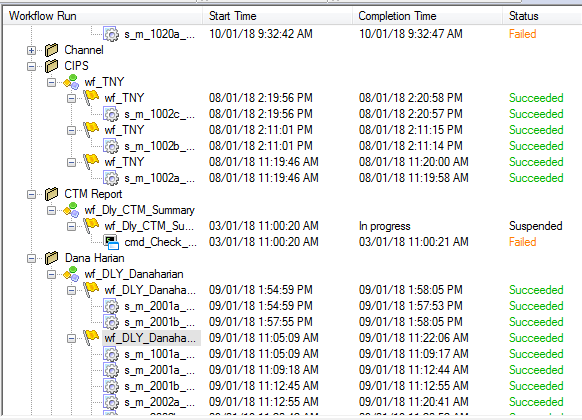
\includegraphics[width=\linewidth]{monitoring-for-report.png}
\caption{SIT process}
\label{fig:sitinfa}
\end{figure}

When doing SIT process, the workflow that has been running needs to be monitored. Figure~\ref{fig:sitinfa} shows the monitoring step of every jobs that has been running. Each workflow that has been triggered to start will show up in this monitoring page. We then make sure the amount of rows that inserted to target table is right and there is no error.\\

As we can see in Figure~\ref{fig:sitinfa} on Status field, the status will said ``Failed'' and suspend the execution if there is an error either in mapping or session settings. The status will come to ``Succeeded'' if there is no error during process of the running workflow.

\subsection{Data Regression}

\begin{figure}[H]
\centering
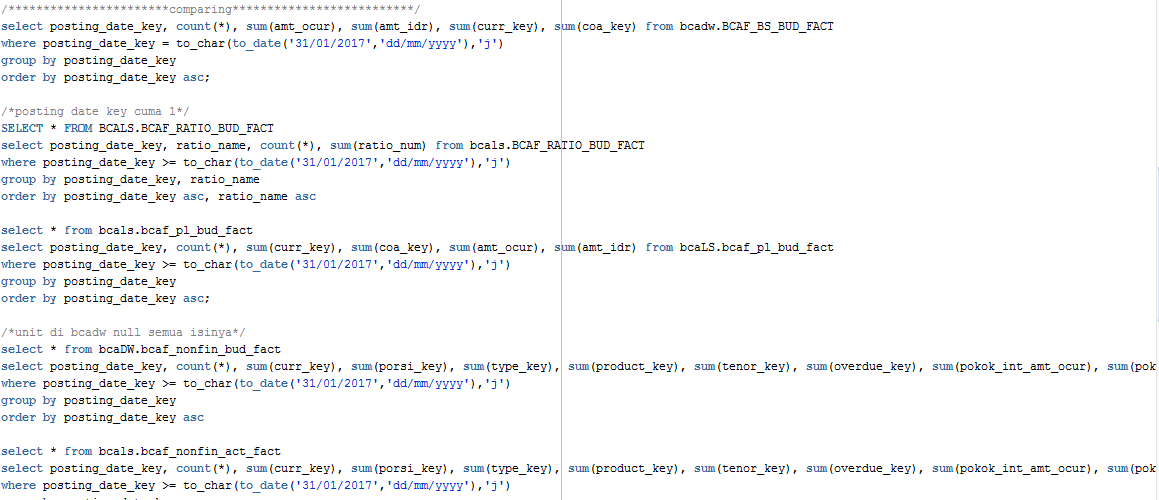
\includegraphics[width=\linewidth]{regresi-for-report.png}
\caption{Workflow in Informatica}
\label{fig:datainfa}
\end{figure}

This step is where datas will be compared. The data from production server (current latest data) will be compared with data from execution of workflow that has been developed (Same source as production's).

\subsection{Implementation}
In this step, every process above has already been completed. This step is where the project that has been developed in development server will be deploy to production server, or can be said as `go live'. There are some procedure before deploying the project. First, create the remedy (a log book/summary of the project), a focal point (an ID to distinguished each project), make sure every component that will be deploy not in `check out' condition, and finally the project can be deploy.

\subsection{PIR}
After the project has been implemented, PIR (Product in Review) step is needed to confirmed the project has successfully work according to user requirements. In this step, the user will test the application and comparing the data in the application and in data warehouse. If it's same, then the project is done and closed. If not, it will be develop again to find the mistakes.

\section{Task Completion and Problem Handling}
In 6 months of doing internship in BCA, the author jobs is to create the ETL jobs either based on pure query script or from old ETL jobs mapping. Besides the migration, the author also assist some of other collage's projects. For instance, the author helps develop projects that involves some changes on certain tables.\\

The author also was given a project that isn't involved in database, which is fulfilling the audits demands. The audits want a whole network architecture in DWH (Datawarehouse) Team. In this project, the author was assigned to create the network architecture in production server for audit people. In this project, the author needs to know which server that is currently still being used/running and which server that already outdated. To know this, the author ask every PIC on an application/software that's been used in DWH team.